\documentclass[9pt, technote, a4paper, nofonttune]{IEEEphot}
\usepackage{wrapfig}

\jvol{xx}
\jnum{xx}
\jmonth{March}
\pubyear{2023}

\newtheorem{theorem}{Theorem}
\newtheorem{lemma}{Lemma}

\begin{document}

\title{D5: Team J Smart Meter Design Final Report}

\author{Yai Sagolsem (ys6g21), Mathyus Marshall-Panayiotou (mmp1u19), Islombek Karamatov(ik5g21), AoYang Leng (al7g20), Yiyang Hu (yh10u21), Gagan Vithanala (gv4g21)}

\affil{University Of Southampton, Electronics and Computer Science}
\maketitle
\vspace*{-96pt}
\begin{figure}[h!]
    \centering
    
\includegraphics[width=20pc]{D5/University symbol.png}
\end{figure}\vspace*{-48pt}
\markboth{ELEC2217}{Electrical and Electronic Engineering Design}
\begin{receivedinfo}%
\end{receivedinfo}
% Contents
\begin{center}
\tableofcontents
\end{center}
\vspace*{24pt}
\begin{figure}[h!]
    \centering
    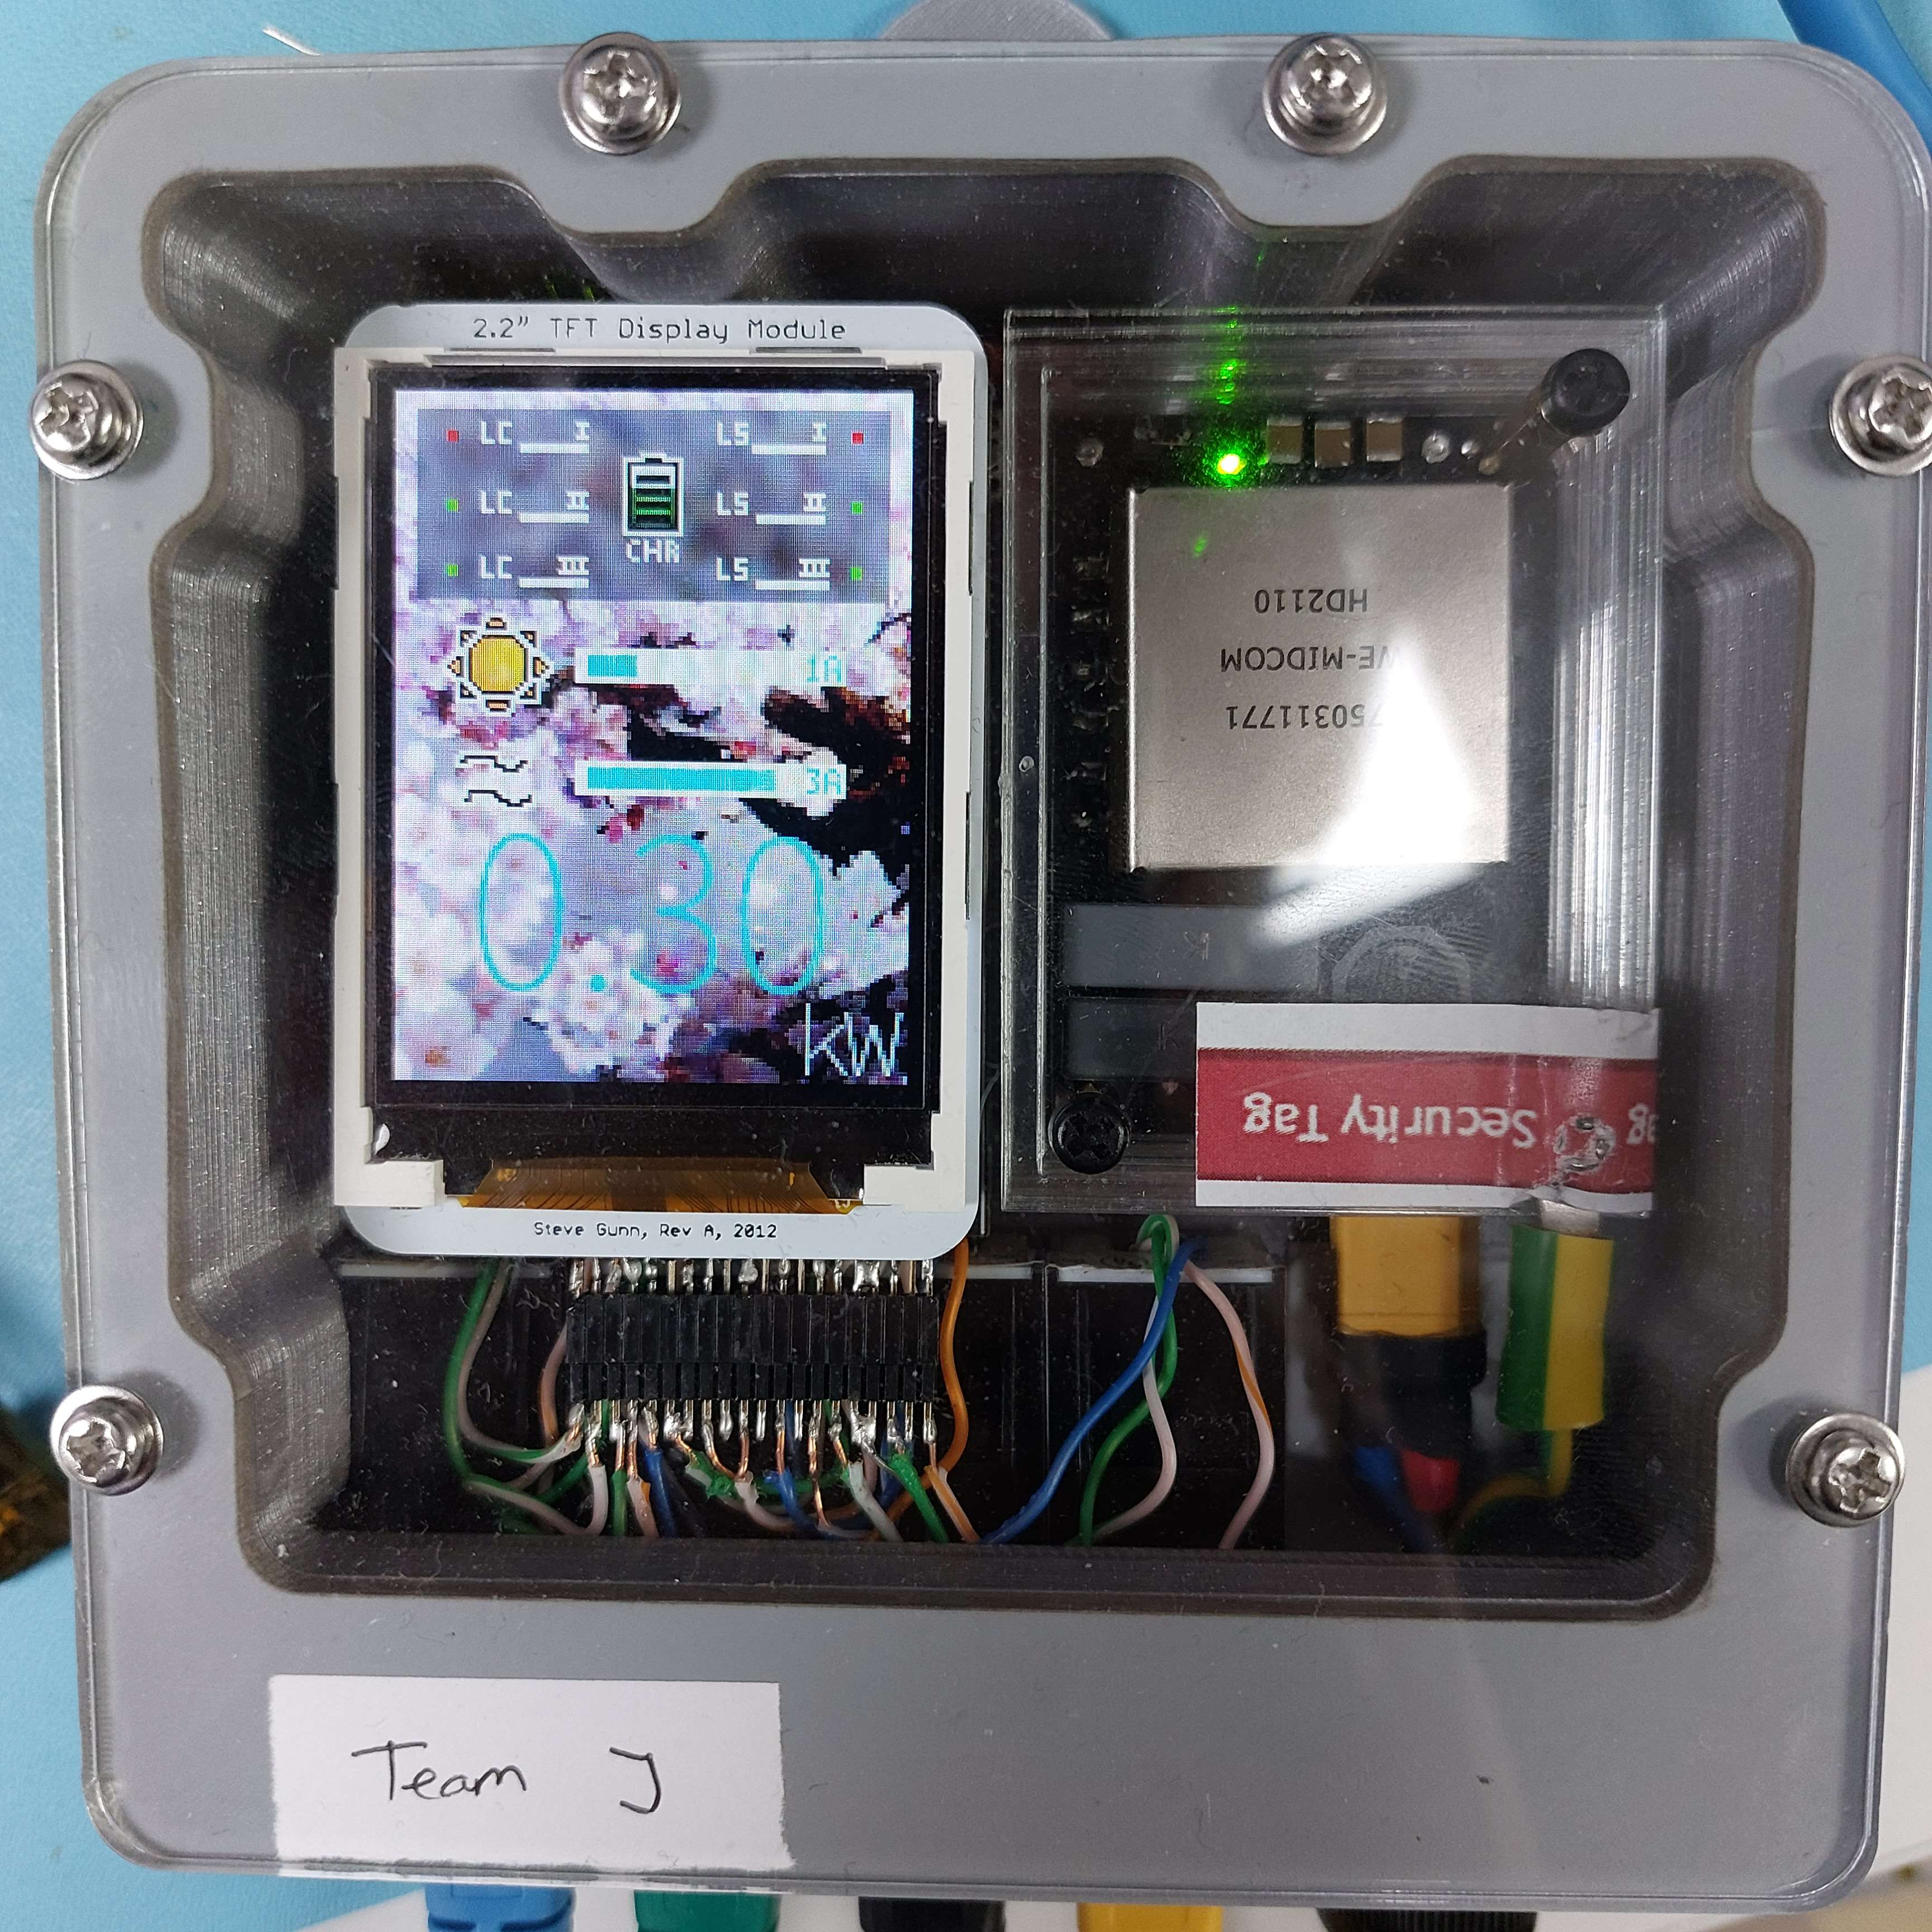
\includegraphics[width=35pc]{D5/SmartMeter1.jpg}
    \caption{Our final smart meter design in operation.  Load switch and call indicators visible, alongside the two PV and  Wind level power bars.  Beneath is the large total power readout}
\end{figure}

        

\newpage
\section{Introduction and Project Vision}
\hspace{0.5cm}Our team began the D5 Smart Meter Project with good enthusiasm and a drive to accomplish more than what was expected.  This report will document the design that was produced and the final outcome and reality of that initial enthusiasm as it was tested against the many unfortunate obstacles that presented themselves.

\section{Team Roles and Coordination}

\textbf{Gagan Vithanala (gv4g21)}:  Initially assigning themselves to working on the housing, Gagan helped to design and validate the design that was eventually produced, by producing accurate CAD models of the various connectors.  After the housing was completed, Gagan helped to design some of the LCD iconography.
\\
\\
\textbf{Yiyang Hu (yh10u21)}:  Yiyang was initially the main lead for housing design, and worked with Gagan to produce the designs for the first review.  Afterwards, designs were iterated with Gagan under the guidance of the project lead to produce the final housing design.  Once the housing was finalised, Yiyang began to draft the initial pixel dimensions of the LCD graphics.
\\
\\
\textbf{AoYang Leng (al7g20)}:  Aoyang worked with the project lead to develop backup PSU as well as the initial interface circuitry.  Unfortunately some time was lost during the project as Aoyang fell ill for a week.
\\
\\
\textbf{Islombek Karamatov(ik5g21)}:  Islombek worked with Mathyus on the algorithm and software, and also wrote part of the firmware (io.c and mainsreq.c).  Unfortunately during the final weeks Islombek was unable to work on the project extensively for 6 days as he had to travel to Manchester as his Visa was almost invalidated but he still helped with the algorithm development and testing during that period.
\\
\\
\textbf{Mathyus Marshall-Panayiotou (mmp1u19)}:  Mathyus was the main software lead and worked extensively on the algorithm with Islombek, and worked with the project lead to integrate it with the firmware.  Unfortunately during the last few weeks Mathyus also fell ill with Aoyang and was also unable to attend meetings.
\\
\\
\textbf{Yai Sagolsem (ys6g21)}:  With the most practical and software experience, Yai acted as the main project lead, overseeing all areas of the project, especially electrical, providing guidance and design improvements when necessary.  Yai also wrote most of the firmware as well as the LCD driver.  The project source can be found on Yai's GitHub at https://github.com/kaichodesu/sotond5


\newpage
\section{Power Supply}
        \subsection{Initial AC to DC Regulation}
        \hspace{0.5cm}Many designs for AC to DC regulation were considered, however, with the restrictions of size, cost, efficiency and safety, the main options presented were swithmode topology designs such as switched inductor or switched capacitor.  Upon extensive simulations using PSpice with industry standard software such as Cadence's OrCAD, a great effort was made to produce a finished schematic and PCB that would be manufactured once and work flawlessly the first time.
        \subsubsection{Primary Side Regulated Flyback Topology}
        \hspace{0.5cm}A PSR flyback converter based around the Texas Instruments UCC28730 flyback controller was chosen as it would provide full galvanic isolation while also using a secondary side wake-up monitor to allow for reduced low load parasitic power losses.
        \subsubsection{Optimising for Low-Load Efficiency}
        \hspace{0.5cm}As a typical flyback converter is optimised for high load efficiency, our design had to be manually tuned with ZVS snubbers and careful simulation of MOSFET dv/dt to pinpoint component values that allowed us to avoid having to snub inductor voltage spikes where possible - greatly reducing the amount of energy lost while under low power conditions.
        \subsubsection{Capacitor Discharge Requirements}
        \hspace{0.5cm}Unlike most AC to DC designs, we were able to greatly reduce our required input capacitance by many orders of magnitude - only using an input capacitance of 300 nanofarads.  This allowed us to easily satisfy the safety capacitor discharge requirements, our voltage dropping below 30V upon mains disconnect almost 
        instantaneously.
        \begin{figure}[h!]
            \centering
             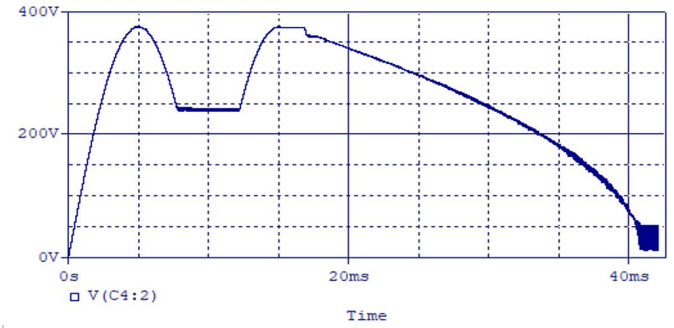
\includegraphics[width=20pc]{D5/CapDischarge.png}
            \caption{Full discharge in less than 50 milliseconds.}
        \end{figure}
        \subsubsection{Schematics}
        \begin{figure}[h!]
            \centering
             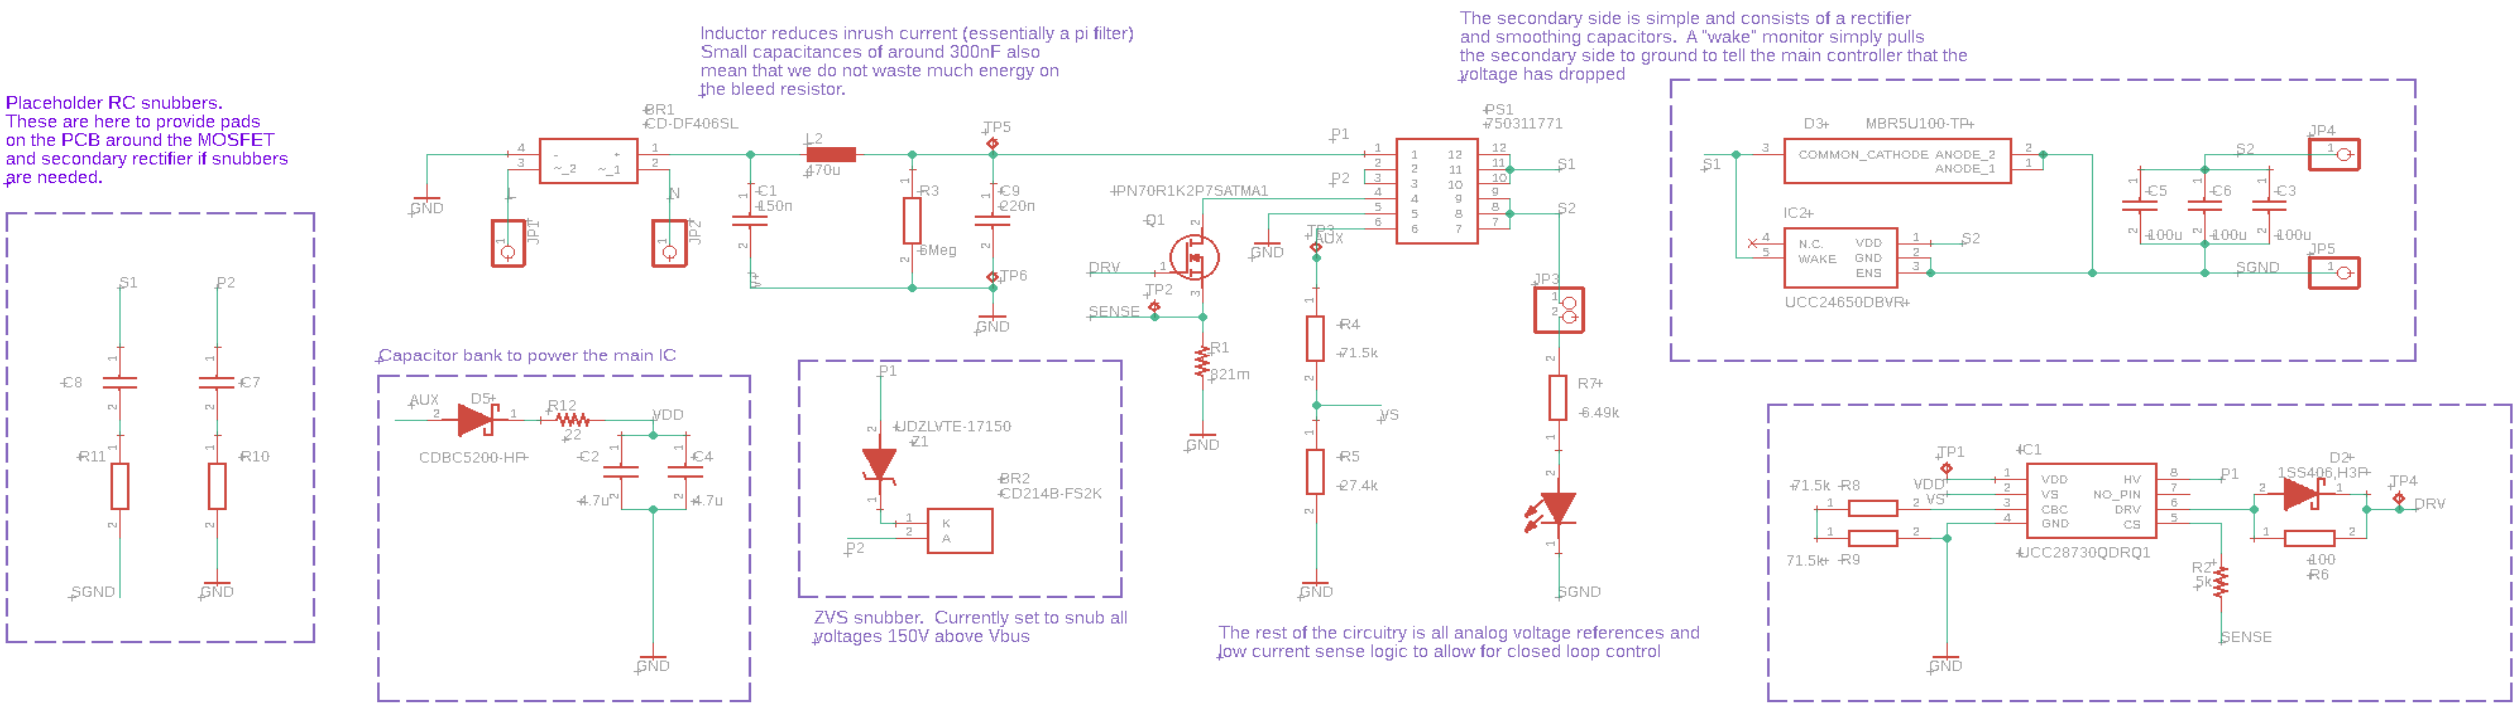
\includegraphics[width=35pc]{D5/Schematics psu.png}
            \caption{The Final PSU Schematic.}
        \end{figure}

\newpage
\section{Interface Circuitry}

        \subsection{Introduction of Interface Circuitry}
        \hspace{0.5cm} In order to connect the Test Bed to the smart Meter, an interface 
        circuit system must be built, which consists of 8 small circuits in total. They are 
        all signal processing problems about voltage transform. Four significant sections 
        called Analogue input, Analogue output, Digital input, and Digital output. All input 
        sections need to convert voltage from Smart Meter to the Test Bed and the output 
        sections from the Testbed to Smart Meter.
        
        \subsection{Analogue Input}
        \hspace{0.5cm} The main capacity in the analogue input section asks us to give the 
        Test Bed a DC 0~10V voltage. Figure 1 shows that R1 and C1 convert the pulse to DC 
        voltage, and the non-inverting Operation-Amplifier output the 10V DC voltage. PSU 
        provides 15V to Op-Amp.
        \begin{figure}[h]
        \centering
        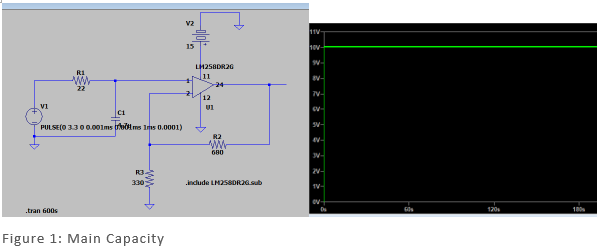
\includegraphics[width=30pc]{D5/3.3v (main capacity).png}
        \label{fig_env1}
        \end{figure}
        
        \subsection{Analogue Output}
        \hspace{0.5cm}As part of the Analogue output, a busbar voltage should have a stable 
        output of 3.3V from AC -4V to 4V, as seen in Figure 2. Using one inverting Op-Amp 
        and one voltage follower to get the correct result. PSU provides 15V to Operation-
        Amplifier. One diode to convert AC to DC. One capacitor makes output voltage more 
        stable. Furthermore, as busbar current circuit was also made from AC - 10V~10V to 
        3.3V, figure 3. The circuit is similar to the busbar voltage. Moreover, Wind and PV 
        capacity circuits from DC 0V~5V to 3.3V are similar to the Digital output section, 
        which will be introduced later, shown in figure 4.\vspace*{-6pt}
        \begin{figure}[h]
        \centering
        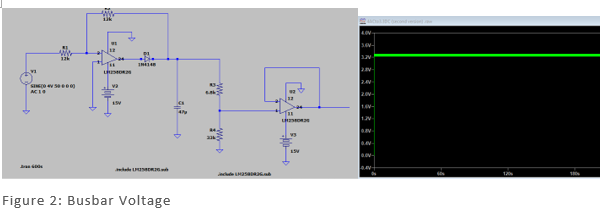
\includegraphics[width=30pc]{D5/4AC.png}
        \label{fig_env1}
        \end{figure}\vspace*{-6pt}
        \begin{figure}[h]
        \centering
        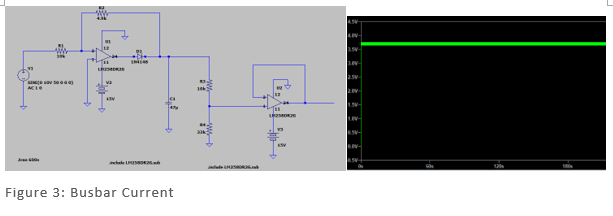
\includegraphics[width=30pc]{D5/10AC.png}
        \label{fig_env1}
        \end{figure}\vspace*{-12pt}
        
        \subsection{Digital Input}
        \hspace{0.5cm} Regarding the TTL logic voltage signal, the voltage needs to be 
        transformed to a square signal 0~5V from the 3.3V Smart Meter for the Digital input 
        section. In the TTL logic signal, 5V logic high means turn on, and 0V logic low 
        means turn off. Our group decides directly output it from il Matto.

         \subsection{Digital Output}
         \hspace{0.5cm} The last part is also about the TTL logic signal, which is from the 
         Test Bed 0~5V to Smart Meter 3.3V. Hence, it has the same principle as the Wind and 
         PV capacities in Analogue output. Similar circuit with a different source. Just a 
         simple voltage follower.
        \begin{figure}[h]
        \centering
        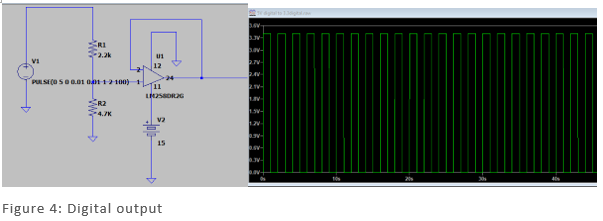
\includegraphics[width=30pc]{D5/5 digital.png}
        \label{fig_env1}
        \end{figure}

\newpage
\section{Physical Design}

        \subsection{Housing and CAD Modelling}
        \subsubsection{Intro to Housing Design}
        \hspace{0.5cm} The enclosure design needs to be convenient, waterproof and have clear viewer visibility of the readings on the LCD screen. It needs to implement these core principals along with the requirements stated in the specification. The box is limited to a 110x110x110mm dimension which should consist of a minimum of three parts. It needs to include a mounting lug so it can be hanged and five RJ45 ports along with a cable gland port. Lastly, the design should allow for easy access (within a minute) to the internal circuitry and needs to incorporate a segregated area for the PSU to prevent it from interfering with the other circuitry. The final design is influenced by outdoor socket enclosures, having a compact design and the use of O-rings and gaskets. The design consists of 4 parts: acrylic lid, main box, the electronics tray, and the PSU enclosure.
        \\
        \begin{figure}[h]
        \centering
        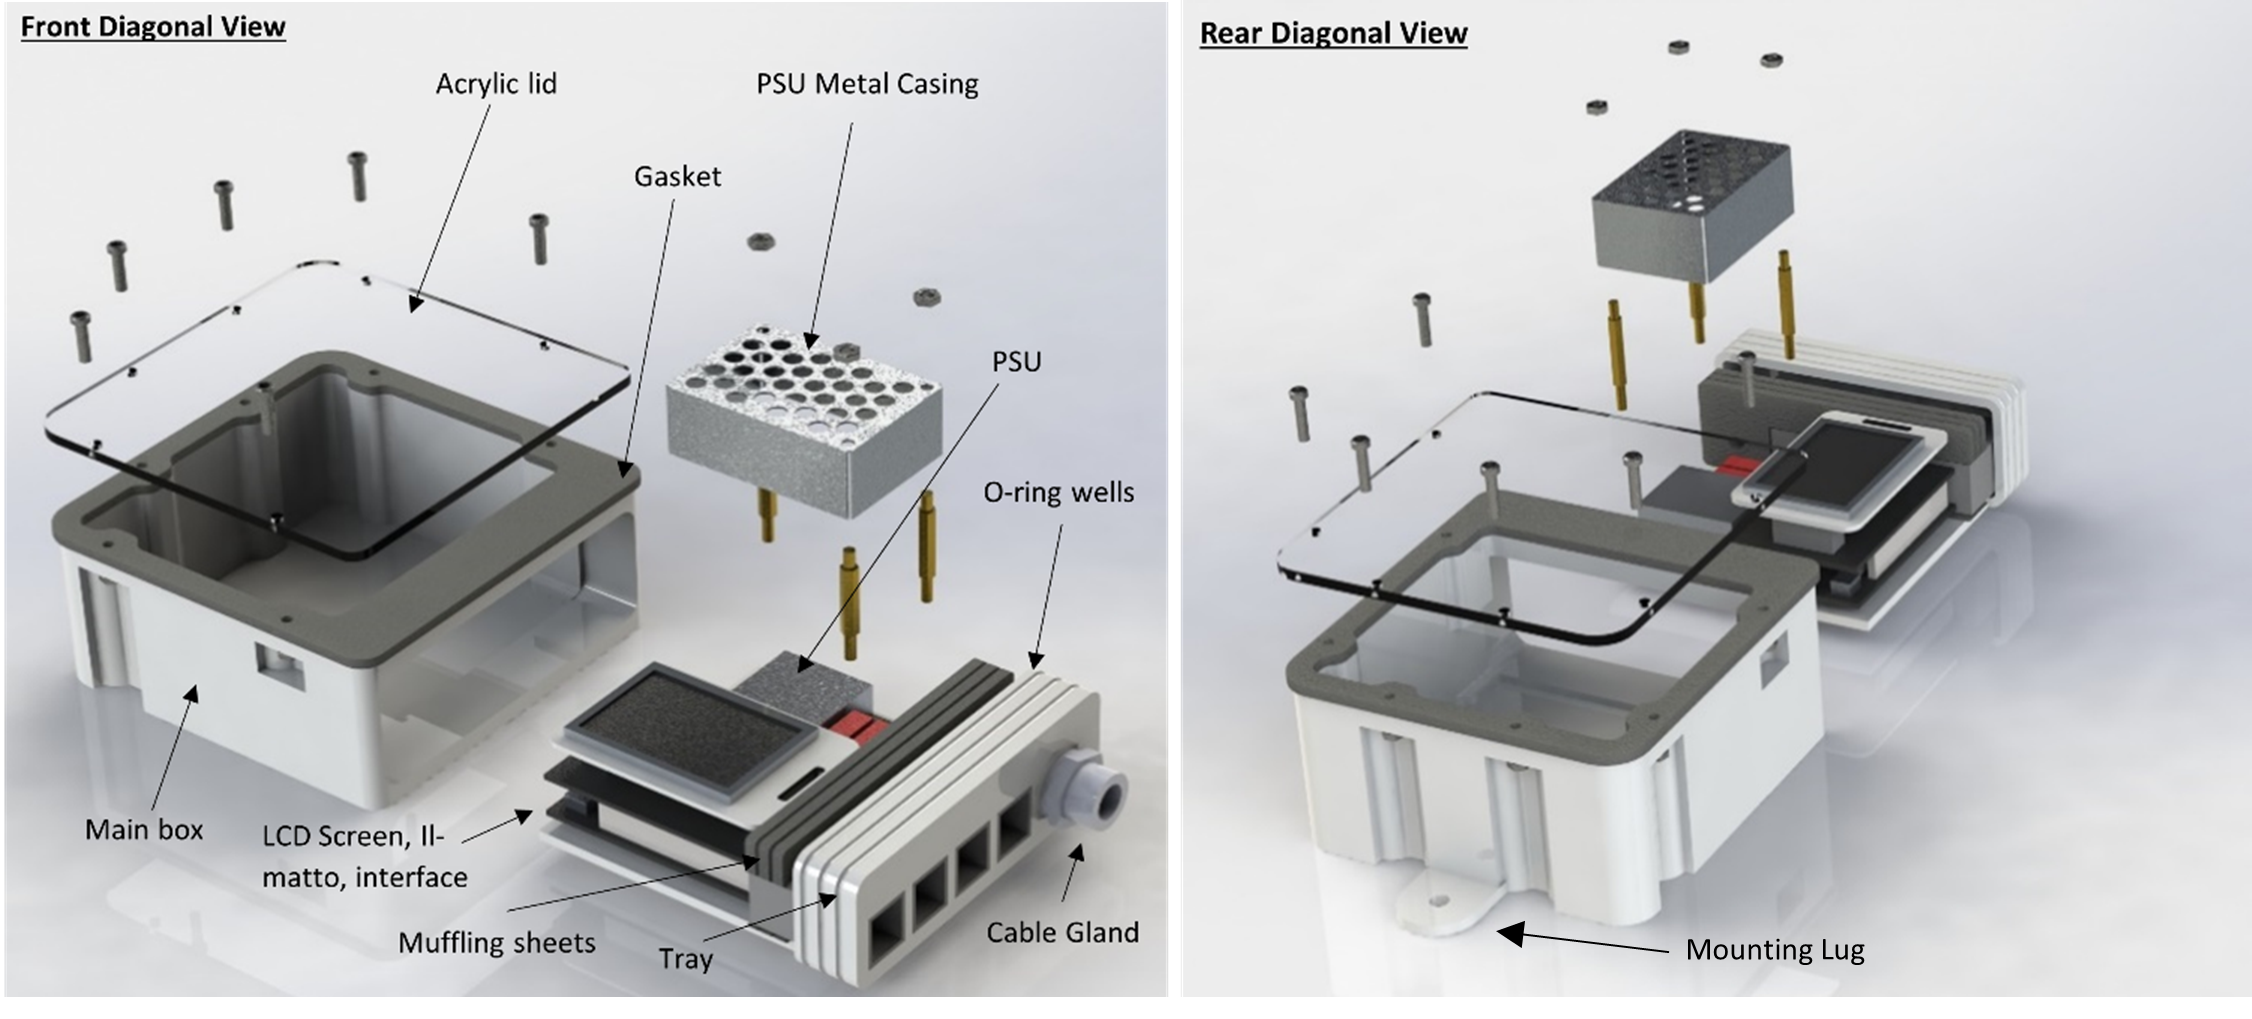
\includegraphics[width=30pc]{D5/Enclosure3DModel.png}
        \caption{3D SolidWorks Exploded view of Housing}
        \label{fig:x Enclosure}
        \end{figure}
        
        \subsubsection{Acrylic Lid}
        \hspace{0.5cm}The final box uses a laser cut acrylic lid on top. This allows the user to read information displayed on the LCD screen and plays its part in the box aesthetic, being able to see the circuitry inside. It aids with the tray mechanism too as everything is connected on the tray, rather than having the LCD attached to the main body surface, and therefore can be taken out from the box with ease.



        \subsubsection{Main Body}
        \begin{figure}[!tbp]
        \centering
        \begin{minipage}[b]{0.5\textwidth}
        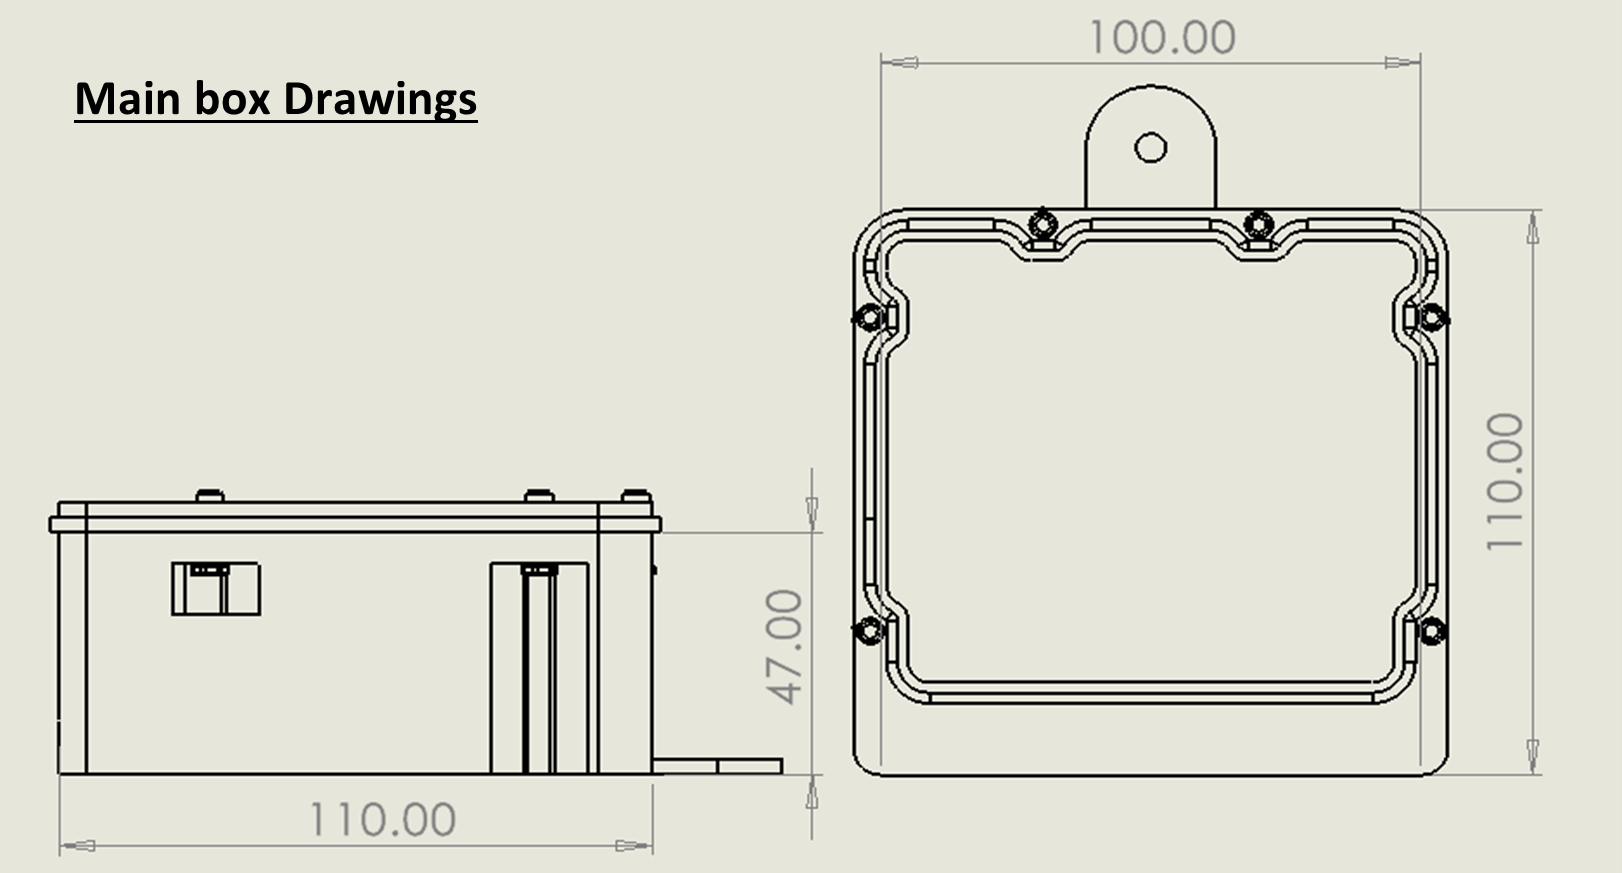
\includegraphics[width=\textwidth]{D5/Main Box.png}
        \caption{Main box drawing}
        \end{minipage}
        \hfill
        \begin{minipage}[b]{0.23\textwidth}
        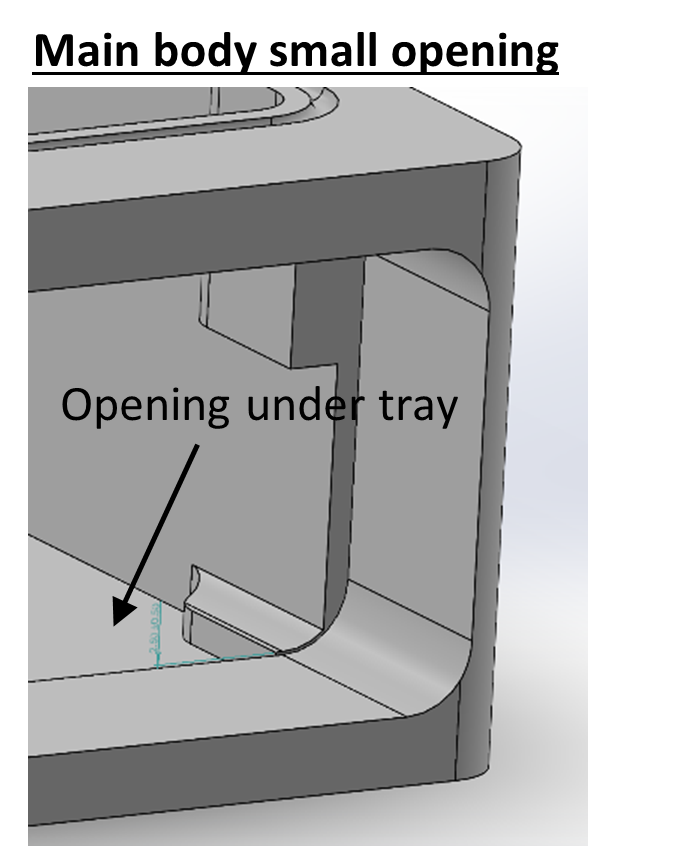
\includegraphics[width=\textwidth]{D5/MainBody_lowerfloor.png}
        \caption{Gap below tray}
        \end{minipage}
        \end{figure}
        
        This is the main part of the housing that encloses everything. It is designed with screw tunnels which gives enough space for the nuts to be placed for the screws. The tunnels near the entrance tray gap are shorter than the rest to make sure it does not block the far left RJ45 when the tray is slid in. After printing the model, it was noticed that the tray and the main body were not interacting well when assembled and dissembled. This was due to the printing tolerance.This was fixed through sanding the inside well walls and the tray opening hole so the O-rings can fit in. The main body also has a small dip after the opening lip to ensure that the screw-heads which are underneath the tray don't prevent the tray from lying flat against the internal cavity. 
        
        \subsubsection{Electronics Tray}
        \hspace{0.5cm}We looked at various mechanisms from using screws to open the enclosure to a screwless tray mechanism. The tray design seen in figure 1 holds the PSU, Il-matto PCB stacked on Interface board (customised to fit in a compact space), and the LCD screen. Holes are drilled into the tray platform into which M3 screws and standoffs hold the PCBs in position. The tray can be ejected so the circuitry can be accessed. The decision of using no screws, to keep the tray in, allows for us to access the internal circuitry well under a minute. We ensured the tray , when inside the main box, stays and supports the weight with all components with the use of O-rings fitted in the three 1.5mm diameter groves. This means we can use the tension and frictional forces between the tray, O-ring, and the box wall to make sure that the tray stays in when closed.
        Spacing in between cutouts for the RJ45s and the cable gland was a concern. The cut-out positions were determined by building SolidWorks models of the RJ45 and cable gland. 
        \begin{figure}[h]
        \centering
        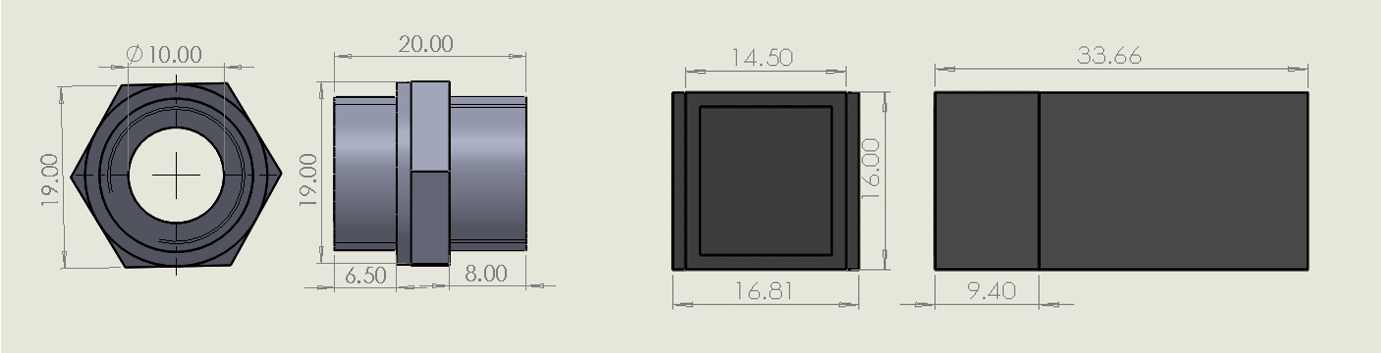
\includegraphics[width=20pc]{D5/CableGland_RJ45_CAD.png}
        \label{fig_env1}
        \caption{RJ45 and Cable gland CAD Models}
        \end{figure}
        \begin{figure}[h]
        \centering
        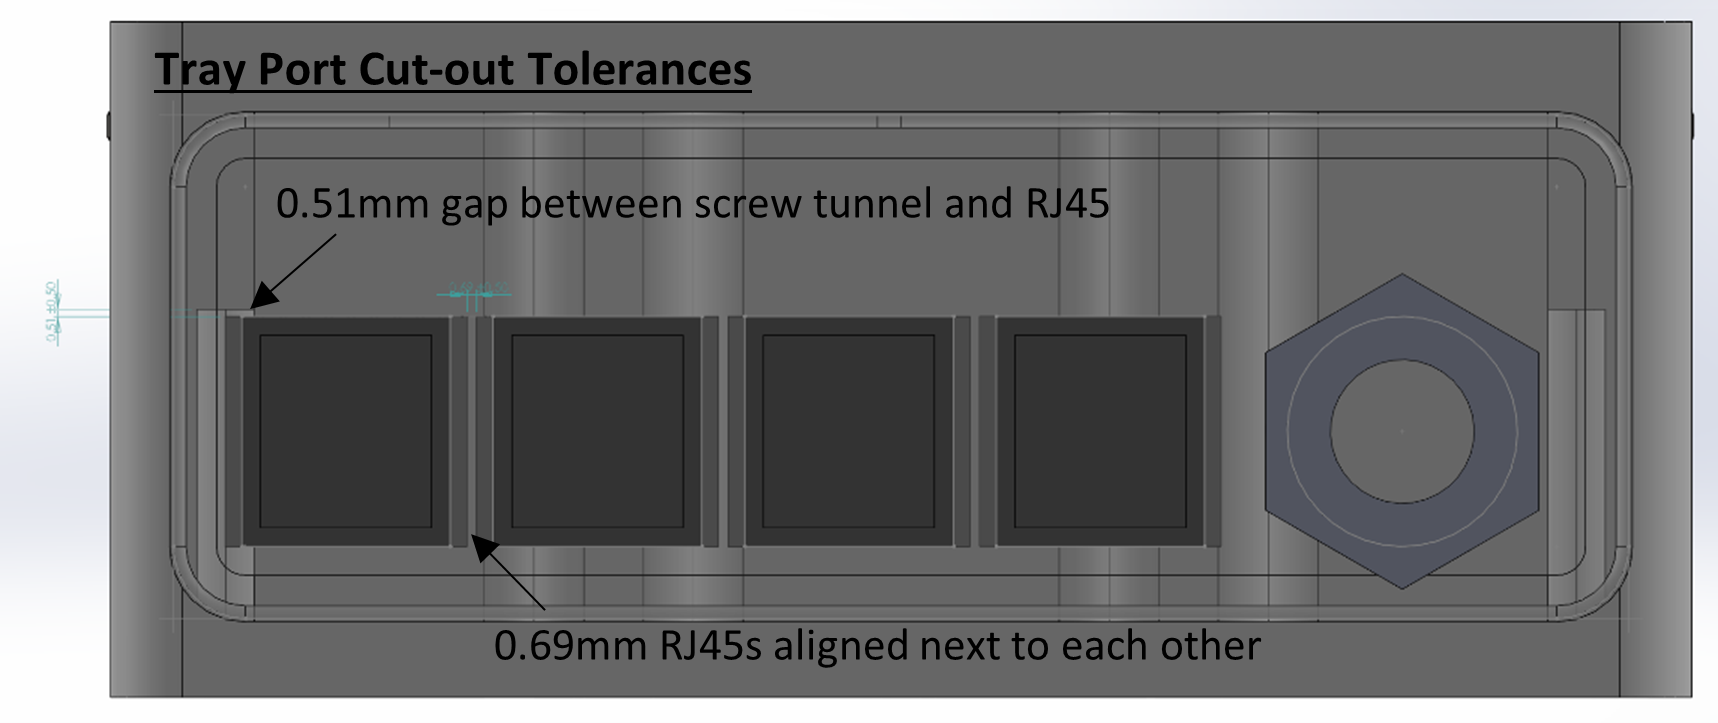
\includegraphics[width=20pc]{D5/Tray Port Cutouts.png}
        \label{fig_env1}
        \caption{Front view drawing of Tray}
        \end{figure}
        \\
        We were tight with a tolerance of 0.69mm. This resulted in the 3D printed model to just about fit all the RJ45s beside each other with no minimal gap.
        
        

        \subsubsection{Waterproofing}
        \hspace{0.5cm}Gaskets and O-rings are mainly used for waterproofing. A gasket is used in between the acrylic lid and the main box. These three parts are fixed together tightly using M3 screws and nuts, ensuring minimal water ingress  within the gap. Three laser-cut gaskets are used as muffling sheets which are placed around the Ethernet ports and cable gland to stop any water leaking through the cut-outs. These design choices have proved themselves handy as we got a result of 0mm in the water test, proving the housing is highly waterproof.


        \subsection{PCB Layouts and Manufacture}
        \begin{figure}[h!]
            \centering
             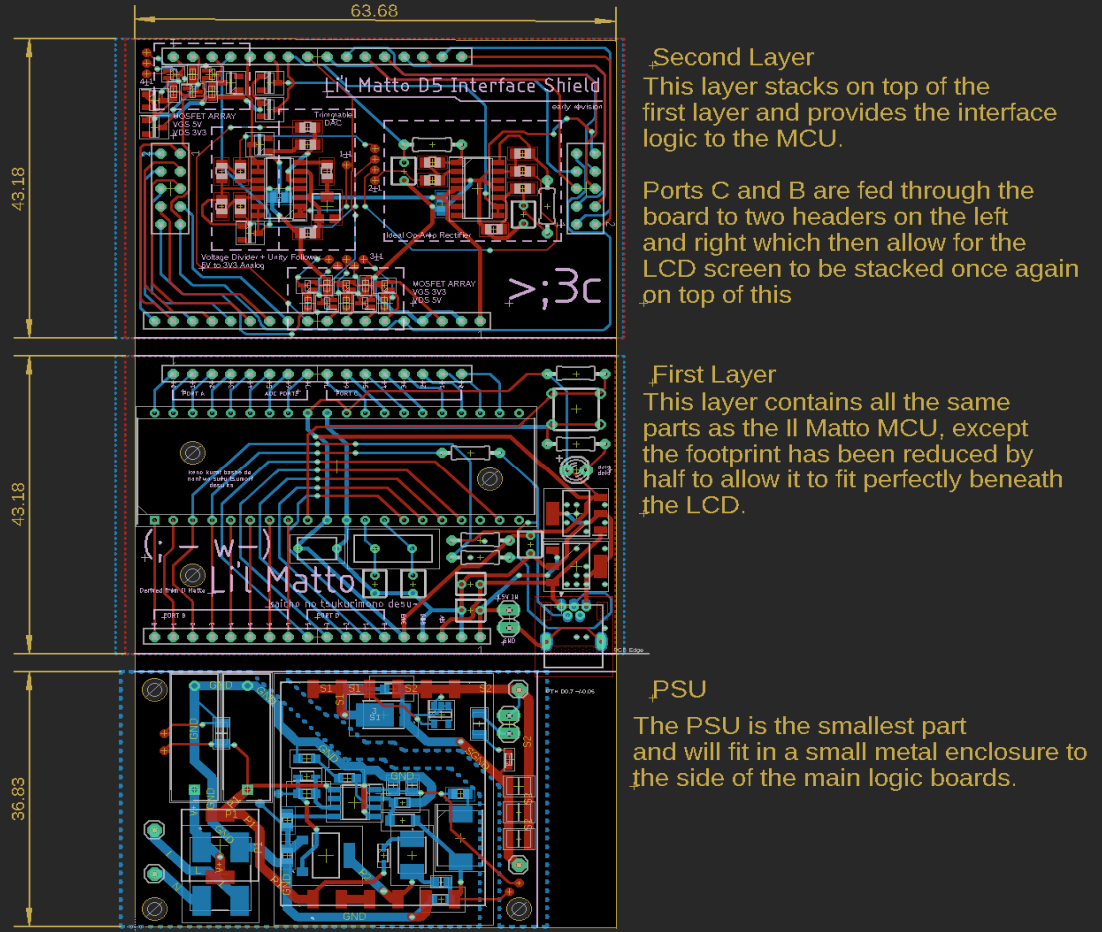
\includegraphics[width=35pc]{D5/PCB layout.png}
            \caption{The final triple board PCB design.}
        \end{figure}


\newpage
 \section{Firmware}
        \hspace{0.5cm}In order to achieve the highest accuracy of data read possible, an advanced firmware had to be designed to run on our micro-controller to provide time-accurate data for the algorithm software to make reliable decisions.  Our firmware was also designed to further limit power consumption as much as possible by using MCU sleep states, further contributing to our incredibly low quiescent power draw.  To limit our BOM, we also opted to use the AtMega1284P as it was already available in the labs, but also featured double the program memory, with 128kB rather than the limiting 64kB that came standard with the Il Matto.

        \subsection{AC Phase Capturing and Clock Alignment}
        \hspace{0.5cm}As our interface design did not use a capacitor to smooth the analog AC signal, we had to initialise a global tick that would send an interrupt at 50Hz to allow our ADC to sample the bus current and bus voltages at the peaks of their cycles.  This was done by initialising one of our 8-bit timers on power up such that it would run at 50.08Hz and send an interrupt whenever its Output Compare Register overflowed.  
        \begin{figure}[h]
        \centering
        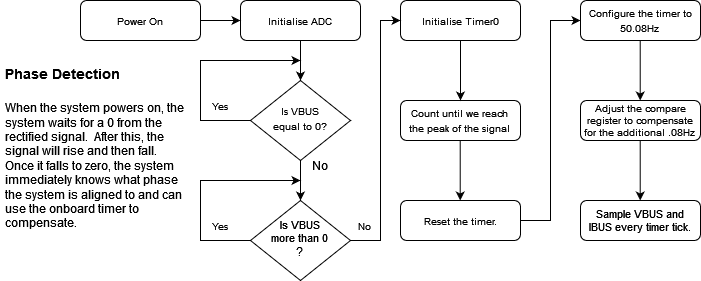
\includegraphics[width=35pc]{D5/System.drawio.png}
        \label{fig_env1}
        \caption{A simplified flowchart of our ADC initialisation.}
        \end{figure}
        \\
        This system essentially acts as a zero-crossing-detector and also allows the system to execute the main software \emph{after} the time-critical bus voltage and bus currents have been measured.  
        \subsection{Noise Rejection}
        \hspace{0.5cm}Due to the large amount of electrical appliances in the testing area, we discovered very quickly that it would be necessary to implement some filters in programming to mitigate the effects of these noise sources.\\Thankfully, the implementation of these filters was relatively simple as the only consideration that had to be taken was to ensure that the total thread execution time did not exceed 10 milliseconds as this would mean the system would overrun its internal 50Hz tick.

        Thankfully, due to the relatively high sampling frequency of the system, it was found not necessary to implement these filters during normal operation, as taking an average of five consecutive readings was enough to nullify any random spikes.

        However, due to the time-sensitivity of the phase detection code, we had to implement a for loop during each ADC event that would write the ADC results to a 20 value array.  As we did not care for the \emph{true} magnitude of the reading - since this was only to detect a zero-crossing - we simply had to make sure that any datum that was disproportionately large to the rest of the values in the array were ignored.
        
        \subsection{MCU Sleep States and Efficiency}
        \hspace{0.5cm}By utilising the aforementioned 50Hz timer interrupt, not only do we ensure that our entire systems operates with up-to-date data, but we can also utilise the deterministic nature of this process to save power when the system is idle.
        Since we can observe how long instructions take to complete, we can then, when possible, put our micro-controller to sleep at the end of the thread, rather than have it constantly operating at full load, constantly sampling for an input that isn't going to change.  Instead, we use the Timer0 Interrupt as a signal to wake the MCU and compute \emph{only when required}, reducing the power consumption of our MCU by up to 80\%.
        \begin{figure}[h]
        \centering
        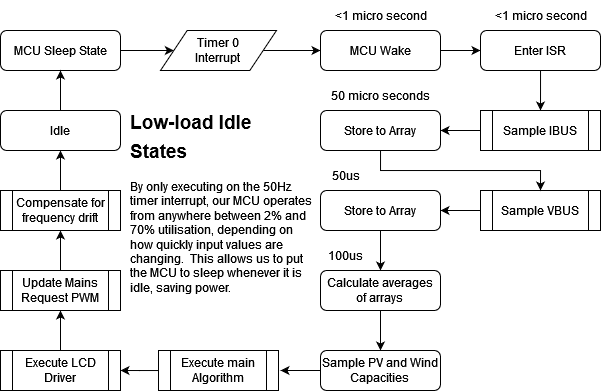
\includegraphics[width=30pc]{D5/Interrupt Service Routine.drawio.png}
        \label{fig_env1}
        \caption{A simplified flowchart of our Interrupt Service Routine.}
        \end{figure}
        \subsection{Display Driver}
        \hspace{0.5cm}In order to display appealing graphics to the end user, we had to design an LCD driver that would not only allow us to directly address the LCD driver chip's data registers, but also do so in a way that did not compromise the timing cycles of the Phase-Synced interrupts.
        We found that the display instructions took a few hundred milliseconds to execute if we were to update the entire screen, which would prevent our algorithm from running effectively as it would delay the reading of the ADC and thus provide erroneous data for the calculations.
        Thus, we decided to implement an LCD driver that dynamically updates parts of the screen only when necessary.
        \begin{figure}[h]
        \centering
        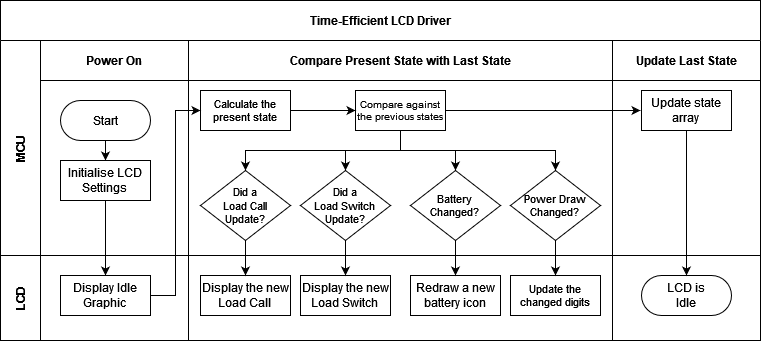
\includegraphics[width=30pc]{D5/LCD timing.drawio.png}
        \label{fig_env1}
        \caption{A simplified flowchart of our LCD Driver.}
        \end{figure}
        \\
        This allowed us to update parts of our screen at 50Hz, after the phase-aligned ADC measurements had been taken - giving the user a smooth visual indicator of our smart meter's actions.
        \subsubsection{Memory Addressing and Memory Management}
        \hspace{0.5cm}One hurdle we had to overcome was the difficulty of programming for an 8 bit micro-controller with more than 64kB due to the memory addressing issues present - standard 16 bit values cannot address the higher memory ranges.
        \begin{figure}[h]
        \centering
        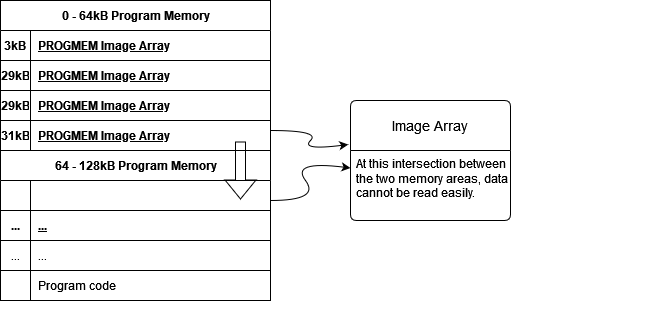
\includegraphics[width=30pc]{D5/memory allocation.drawio.png}
        \label{fig_env1}
        \caption{Highlighting the issues when an image array overlaps the boundary between 64kB and 128kB.}
        \end{figure}
        \hspace{0.5cm}This isn't usually an issue for the end user, however, it was for us since we were storing image bitmap data directly in the program memory, rather than loading it into SRAM as is typically done in normal code.  This issue was eventually overcome by manually searching for the assembly instructions compatible with the 1284P family of micro-controllers and defining macro functions around them to produce a set of functions we could use to interact with data outside the typical 16 bit address range.
      \subsubsection{Texture mapping}
      \hspace{0.5cm}Wanting to make our user interface as appealing as possible, we invested into creating our own font set to display larger, more legible numbers on the screen.  Naturally, this came with a problem that had to be solved by looking at the methods used by developers in the past when once restricted by similar low memory, low processing power environments.
        \begin{figure}[h]
        \centering
        
\includegraphics[width=35pc]{D5/digit2.png}
        \label{fig_env1}
        \caption{A texture containing all the digits used for our power readout.}
        \end{figure}
        \\
    \hspace{0.5cm}Similar to the 8 bit computing era of digital entertainment, we also use texture maps to display our numbers.  Each number is addressed by calling it from its offset, allowing us to then draw the pixels after the offset to display the desired digit.
        

\newpage
\section{Software}
        \subsection{Algorithm}
        The algorithm runs off the basis that each load call can be represented as a binary number. Three loads represents 8 possible combinations of loads being either on or off (000-111). Firstly, we check which combination of loads are on and decide what to do accordingly.
        \subsubsection{Supply and Demand}
       Loads are prioritised according to their number, ie Load 1 takes highest priority and Load 3 is lowest priority. 
       If a combination of loads are on and the energy requirements are not met from renewable energy sources, we begin to request from the mains. Bus voltage will drop when renewable sources are not providing sufficient power, so we increase our request from the mains supply iteratively until the bus voltage is at its normal specified value. The battery discharges to provide extra current if the difference between the max supply and  loads that are currently switched on, are less than the value required to charge the battery.
        \subsubsection{Backup Generator}
       Initially we decided to choose whether to charge/discharge the battery outside of the branches, according to bus current. This worked for load values simulated before the final profile was released, however the algorithm became stuck in a loop, constantly charging then discharging. This happened due to the bus current  decreasing if we choose to discharge the battery, therefore the algorithm would see enough space to charge the battery and repeat.

       We decided to place the decision to charge the battery based on constant load values within each branch. If the condition above is met (max supply minus Loads switched on is less than Battery charge current), we discharge the battery, otherwise we charge it.
        \begin{figure}[h]
        \centering
        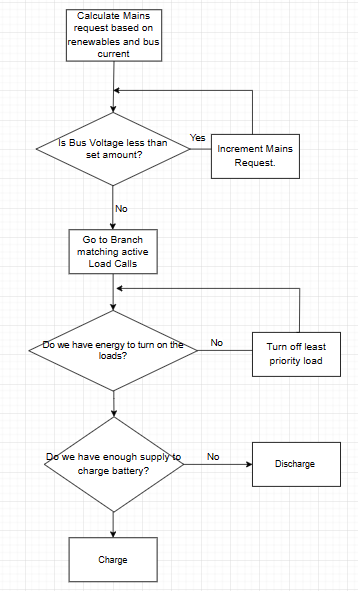
\includegraphics[width=50mm,scale=0.5]{D5/Algo_flow.PNG}
        \label{fig_env1}
        \caption{Simple flowchart showing the basic functions of algorithm.}
        \end{figure}
        \\
 \subsubsection{Equations and conditions}
 The general equation used to calculate how much to request from mains is as follows:

\[ Mainsreq = \frac{10}{MainsMax} *BusI - (PV + Wind) \]

We cannot request a negative amount from mains or above 10, so two simple if statements were used to limit this:
\[if(MainsReq > 10) MainsReq = 10 \]
\[if(MainsReq < 0) MainsReq = 0 \]

Deciding whether to charge or discharge the battery is done using the following general equation and is dependant on what branch of the algorithm we are currently in:
\[if( (MainsMAX + PV + Wind) - sumOfLoads < BatteryChargeI  )\]
\[discharge \]
\[else\]
\[charge\]

fig.16 shows how we choose to turn loads on or off and gives a good description of load call dependant branching.



\section{Conclusion}\vspace*{12pt}

\hspace{0.5cm}Overall this project has been a mixed experience with lots of areas that could have been improved upon.  While there was great opportunity for the development of a truly outstanding design, unfortunately due to a lack of group morale and motivation mixed with poorly timed absences, the workload left for those who remained was simply too great.\\

\hspace{0.5cm}Time was lost chasing red herrings a result of erroneous power readings during the second review and the project lead failed to audit group progress as aggressively as they should have to ensure that the reported progress was accurate to the current state of the project.\\

\hspace{0.5cm}While it could be said that the goals set out were unrealistic for a short project, it is also fair to suggest that, seeing as the final design produced was only a couple days from perfection, had there been less absences, the goals set were wholly achievable.\\

\hspace{0.5cm}However, despite having failed to produce an adequately performant design, the level of complexity and integration achieved in the time frame is at least something that the group can be proud of.
\newpage
%Appendices

\section{Appendices}
\subsection{Meetings and Minutes}
    \begin{figure}[h]
        \centering
        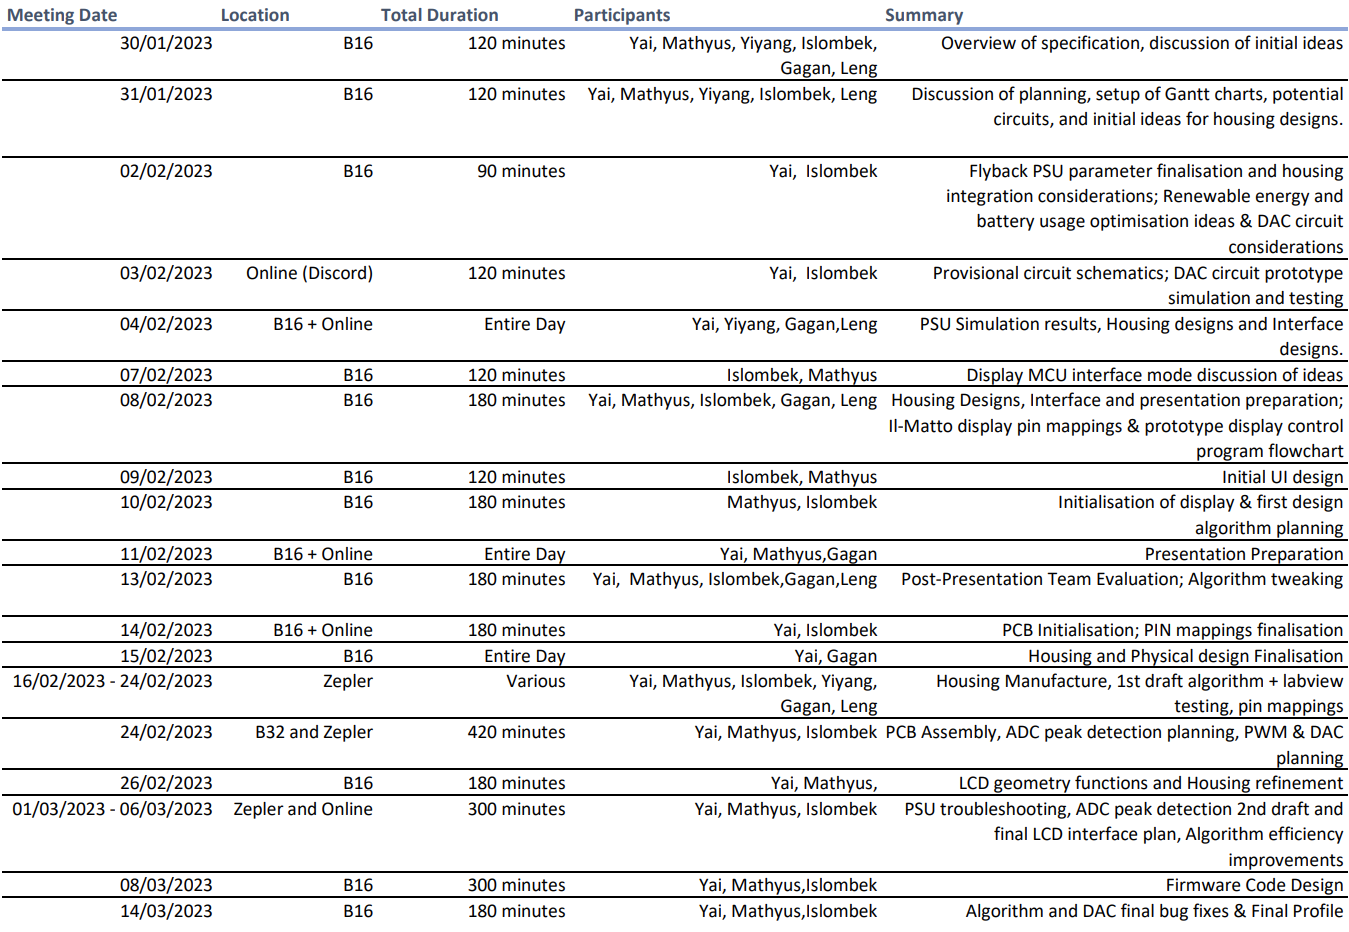
\includegraphics[width=30pc]{D5/Meetings.png}
        \label{fig_env1}
        \caption{A table of our group meetings.}
    \end{figure}
\subsection{Final Bill of Materials and Parts List}
\begin{figure}[h]
        \centering
        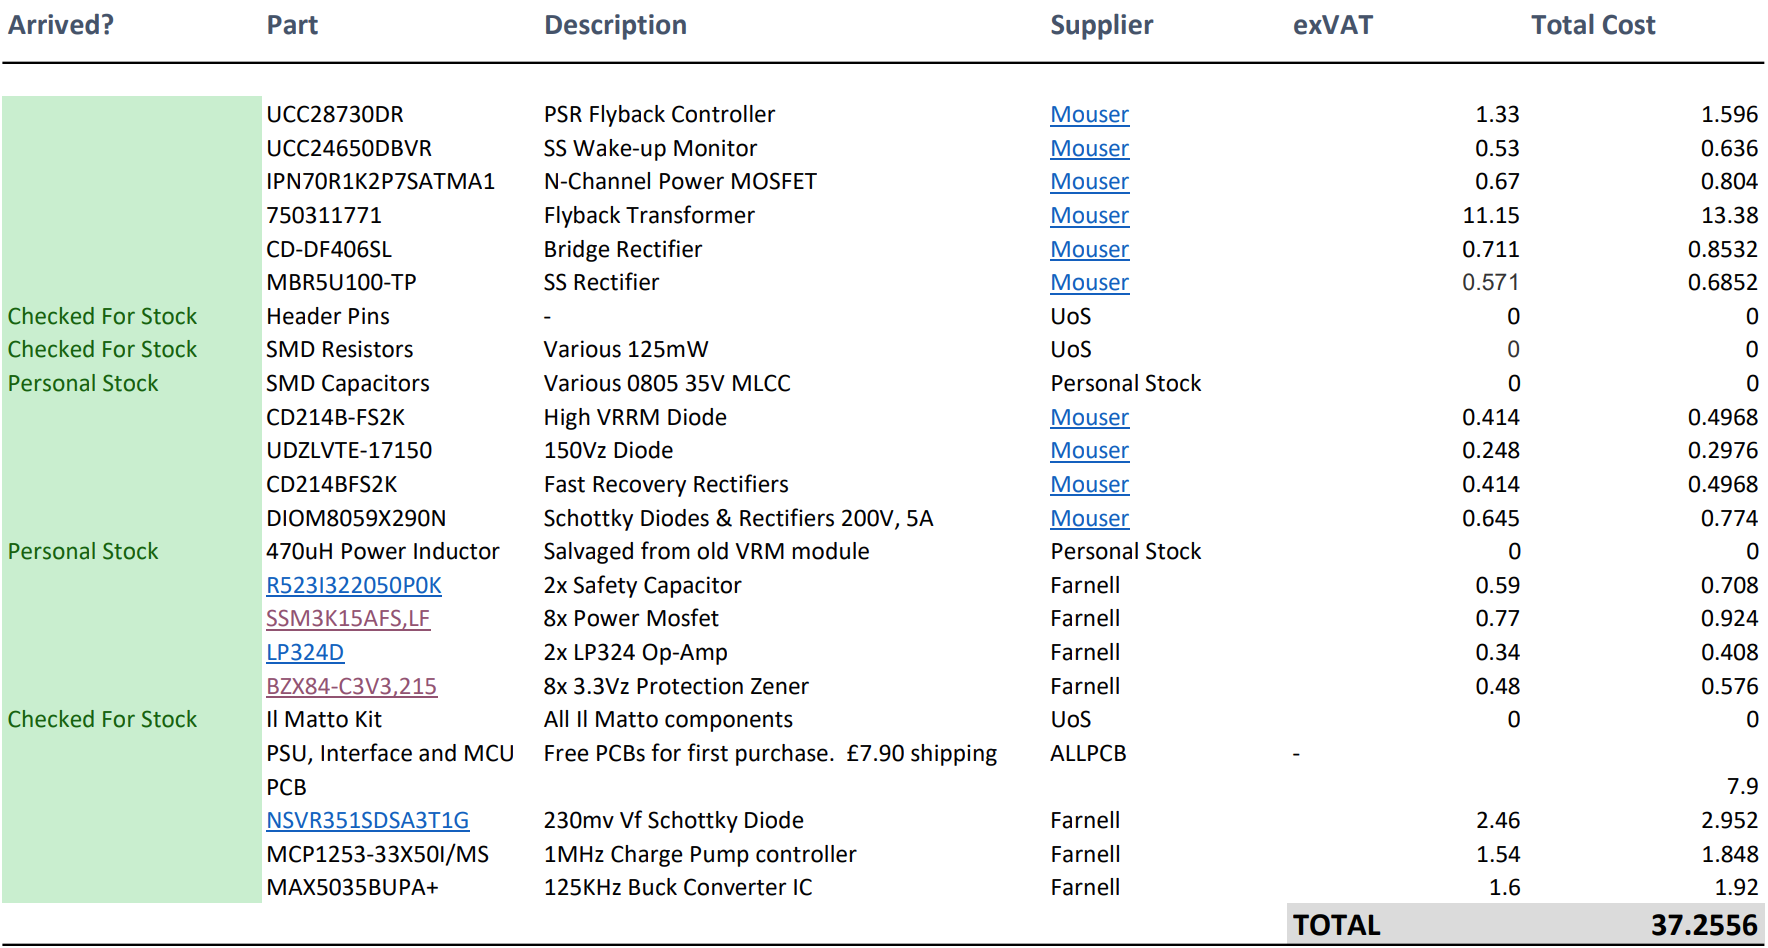
\includegraphics[width=30pc]{D5/BOM.png}
        \label{fig_env1}
        \caption{Bill of Materials}
    \end{figure}

\newpage
\subsection{Team Gantt Chart}
\begin{figure}[h]
        \centering
        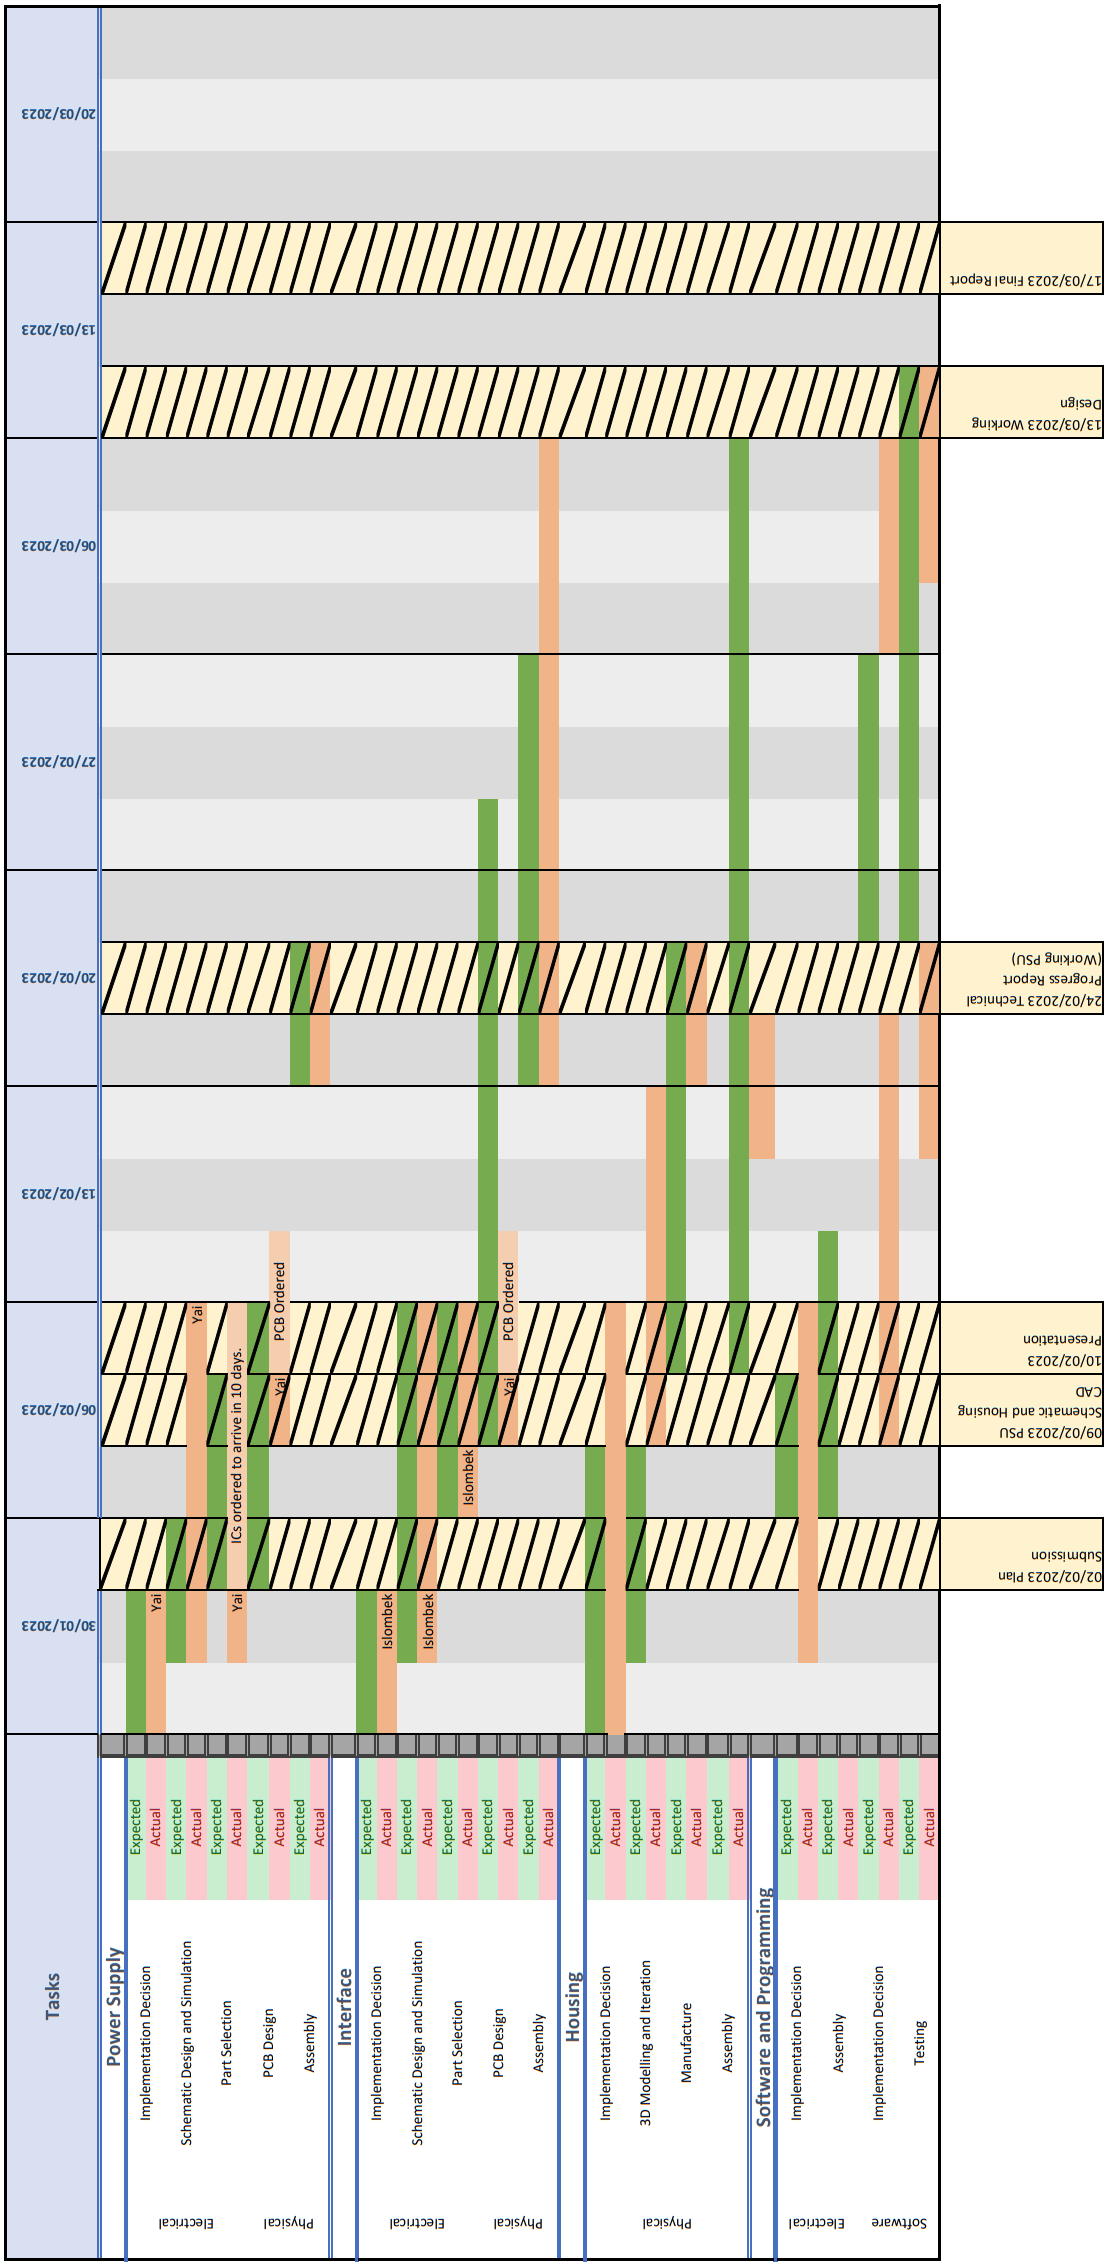
\includegraphics[width=21.5pc]{D5/GANTT.png}
        \label{fig_env1}
        \caption{Final Gantt Chart}
    \end{figure}

\end{document}
